\subsection{Simulation Study}
To validate the variational model, we conduct a simulation study.
    As the problem of multivariate extremes is the estimation of the dependence
    structure of the extremes, we focus the simulation study on on estimation of
    the angular distribution.  The simulated data is generated from a finite
    mixture of projected gammas, at varying levels of dimensionality and number
    of mixture components.  For each simulation, for a \emph{training} dataset,
    \num{1000} replicates are sampled.  For each simulation, for a 
    \emph{testing} dataset, another \num{1000} replicates are sampled using
    the same distributional parameters.

To evaluate the fidelity of our model fitting, we use a generalization of the
    \emph{continuous ranked probability score}, generalized to a multivariate
    setting.  This \emph{energy score} \citep{gneiting2007} takes the form:
    \[
      \text{\makenote{Add Energy Score Equation}}  
    \]
    When energy score is used with an appropriate negative definite kernel 
    metric, it forms a \emph{proper} scoring rule. The specific negative 
    definite kernel we use is developed in \cite{trubey:pg}.   Though geodesic
    distance on $\mathbb{S}_{\infty}^{d-1}$ is computationally inefficient, we
    can find a computationally efficient upper bound on geodesic distance using
    
    
    In Figure~\ref{fig:energyscore} we 
    compare the rise in energy score of the fitted
    model over a \emph{baseline} energy score.  This baseline energy score is so
    called because it is the energy score between a target datase


\begin{figure}[ht]
    \caption{Rise in energy score over baseline (Y) versus dimensionality (X), 
            by number of latent mixture components in generating distribution
            \label{fig:energyscore}}
    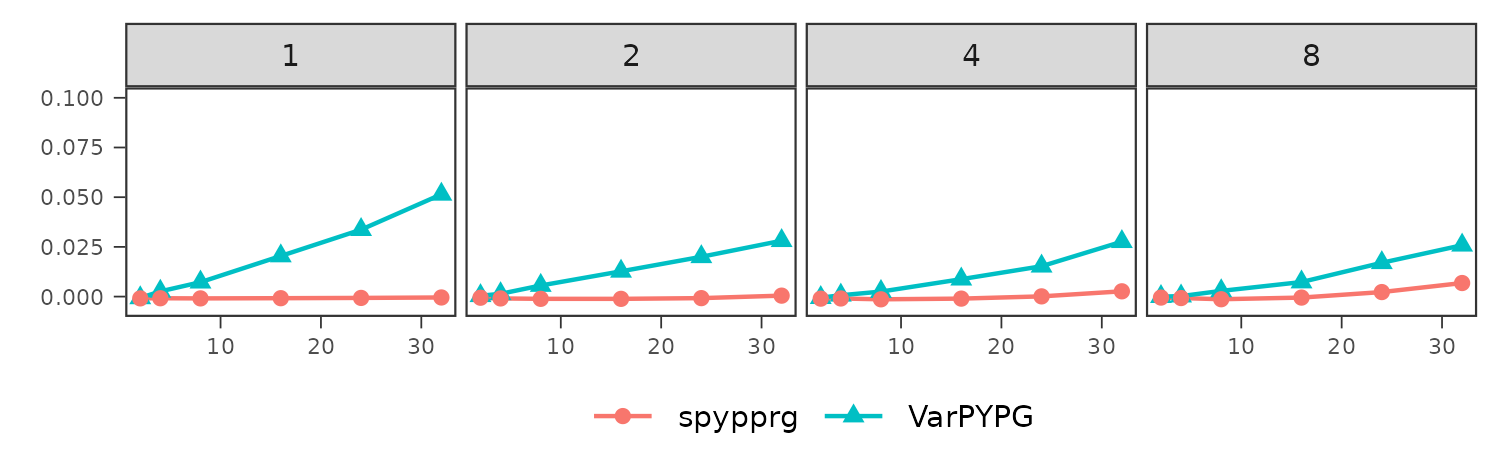
\includegraphics{./plots/energy_score}
\end{figure}


% EOF